\documentclass[letterpaper, 12pt]{article}

\usepackage{geometry}
 \geometry{
 letterpaper,
 total={170mm,257mm},
 left=20mm,
 top=20mm,
 bottom=20mm
 }
\usepackage{graphicx} % Required for inserting images
\usepackage{authblk}
\usepackage{amssymb}
\usepackage{lipsum}
\usepackage{float}
\usepackage{times}
\usepackage{amsmath}
\usepackage[format=plain,
            labelfont={bf,it},
            textfont=it]{caption}
\captionsetup{justification=raggedright,singlelinecheck=false}
\usepackage{ragged2e}
\usepackage{longtable}
\usepackage{comment}
\usepackage{setspace}
\usepackage{fancyhdr}
\usepackage{titlesec}
\usepackage[hyperindex,breaklinks]{hyperref}
\hypersetup{
    colorlinks=true,
    linkcolor=blue,
    filecolor=magenta,      
    urlcolor=blue
    }
% \usepackage{background} % add COSIG logo to page
\usepackage[T1]{fontenc}
\usepackage{helvet}
\renewcommand{\familydefault}{\sfdefault}
\pagenumbering{gobble}
\usepackage[skip=10pt plus1pt, indent=40pt]{parskip}

\titlespacing*{\section}
{0pt}{1.5ex plus 1ex minus .2ex}{1.3ex plus .2ex}

\renewcommand\Authfont{\fontsize{12}{14.4}\selectfont}
\renewcommand\Affilfont{\fontsize{9}{10.8}\itshape}
 
\begin{document}
\flushleft

\includegraphics[width=0.5\textwidth]{img/home/241017_final_logo_mockup.png}

\section*{Getting started with post-publication peer review}
\addcontentsline{toc}{section}{Getting started with post-publication peer review}
\textit{Last updated: 18 June 2025}

Post-publication peer review (PPPR) is an open-ended process with the entirety of the scientific literature in its scope. Be aware that there is no single defined way to get started and no single defined protocol for performing PPPR. Moreover, learning how to do effective PPPR takes time and practice, much like doing good research and good pre-publication peer review. COSIG itself reflects tips and tricks various PPPR practitioners have picked up through their practice.

Remember that performing PPPR is not restricted to identifying problematic articles. PPPR is also a means for furthering discussion on scientific papers on their merits and proposing new perspectives and directions.

This guide covers some suggestions on how to get started if you have not taken part in PPPR before, specifically:

\begin{enumerate}
    \setlength\itemsep{-0.5em}
    \item Decide whether you will perform PPPR under your own name or pseudonymously (your preferences can always change).
    \item Create a PubPeer account.
    \item Start by verifying fingerprints the Problematic Paper Screener has detected.
    \item Start with familiar issues and topics before branching out.
    \item Read other PubPeer comments to learn about interesting cases and best practices.
\end{enumerate}

\subsection*{Accessing articles}

\href{https://en.wikipedia.org/wiki/Open_access}{``Open access''} articles can be read in full by anyone with an internet connection at no cost. Not all articles are open access; many require a subscription to the publisher to read in full, typically provided to academics by their institution. If you do not have an institutional subscription, you may be restricted to performing PPPR on only open access articles and journals. For articles that are not open access, you may only be able to read the title, abstract and author information without cost, often leaving the full text, author declarations and supplementary materials inaccessible. This depends on the article's publisher and when the article was published.
 
Authors sometimes provide PDF copies of their articles on their personal websites or on services like \href{https://www.researchgate.net/}{ResearchGate}. These can be located by looking up the paper title in a search engine.

The full-text of articles in the biomedical sciences may be accessible through \href{https://pmc.ncbi.nlm.nih.gov/}{PubMed Central} or \href{https://europepmc.org/}{EuropePMC}.

Depending on your jurisdiction, \href{https://en.wikipedia.org/wiki/Sci-Hub}{Sci-Hub} and similar file-sharing services for scientific articles may or may not be legal to use.

\begin{comment}

\textit{Be aware that there is no single defined way to get started and no single defined protocol for performing PPPR. Moreover, learning how to do effective PPPR takes time and practice, much like doing good research and good pre-publication peer review. COSIG itself reflects tips and tricks various PPPR practitioners have picked up through their practice.}

\textit{Although anyone can perform PPPR with the right domain knowledge, which COSIG aims to distribute, the best-prepared are working scientists reviewing papers in their career discipline. Remember that performing PPPR is not restricted to identifying problematic articles. PPPR is also a means for furthering discussion on scientific papers on their merits and proposing new perspectives and directions.}

\end{comment}

\subsection*{Anonymity and pseudonymity}

Many choose to perform PPPR anonymously or under a pseudonym. Hiding your identity when performing PPPR can help protect you from harassment, litigation and harm to your career. On the other hand, your name being attached to a review may lend it more credibility. Many publishers, editors and authors will take reviews submitted anonymously or pseudonymously seriously but many others will not (see the section on anonymity in COSIG's \href{https://osf.io/7w5ys}{entry on common dismissive responses to integrity concerns}). Keep in mind that your preference for anonymity can always change--different situations may call for different approaches to sharing your identity.

If you prefer to hide your identity, PubPeer allows users to comment on articles under a randomly-generated pseudonym. Consider creating another email account that cannot be traced back to your identity when sending emails to publishers, editors, and authors. 

If you prefer to guarantee complete anonymity when using any PPPR site or equivalent service, consider hiding your \href{https://en.wikipedia.org/wiki/IP_address}{IP address} by accessing the site via the \href{https://www.torproject.org/}{Tor Browser}.

\subsection*{Create a PubPeer account}

\href{https://pubpeer.com/}{PubPeer} is a PPPR site where users can comment on any scientific article. To date, more than 150,000 scientific articles have been commented upon on PubPeer. It is presently the foremost forum for PPPR and likely the most accessible place to get started doing PPPR.

Go to \href{https://pubpeer.com/register}{PubPeer's registration page} and create an pseudonymous or named account.
You can create as many pseudonymous accounts as you want if you don't want some comments to be linked to the same person.
However, be aware of \href{https://pubpeer.com/static/faq#24}{PubPeer's rules on account moderation}: comments from pseudonymous accounts must undergo moderation before they appear and thus will take longer to be publicly readable. Keep your login credentials secure; you cannot recover an anonymous account if you've forgotten the access code.

Before leaving a PubPeer comment, consult COSIG's \href{https://osf.io/sghaq}{entry on best practices for PubPeer commenting} and \href{https://pubpeer.com/static/faq}{PubPeer's FAQ page}.

\subsection*{Start by verifying fingerprints found by the Problematic Paper Screener}

Problematic articles are often identified because they feature easily-recognizable ``flags'' or ``fingerprints'' that readily indicate that something about the article is amiss. Manually assessing articles with these signatures and commenting on them on PubPeer is an easy way to get started with PPPR, especially for those without scientific backgrounds. Many such fingerprints are compiled by the \href{https://www.irit.fr/~Guillaume.Cabanac/problematic-paper-screener/}{Problematic Paper Screener (PPS)}. The PPS semi-automatically flags tens of thousands of potentially problematic articles across all scientific disciplines. It currently has ten detectors that collect problematic articles featuring fingerprints including \href{https://www.irit.fr/~Guillaume.Cabanac/problematic-paper-screener/tortured}{tortured phrases}, \href{https://www.irit.fr/~Guillaume.Cabanac/problematic-paper-screener/feet-of-clay}{citations to retracted publications} and \href{https://www.irit.fr/~Guillaume.Cabanac/problematic-paper-screener/citejacked}{citations to hijacked journals}. 

The `All Problematic Papers' tab in the left sidebar shows results for all detectors. Clicking on this will bring you to a table of all flagged articles, including their title, venue, publisher, year, as well as which PPS detector spotted issues and what potential issues were spotted.

% To begin with the PPS, go to the ``All problematic papers'' tab on the left:

% Not really necessary, as the screenshot is just 'All Problematic Papers'
%
\includegraphics[width=0.4\linewidth]{img/getting_started/AllProblematicPapers.png}

If you are interested in a specific kind of article (such as articles from a particular publisher), you can click on the title of a column to filter it, and search within that filter for what to pick:


\includegraphics[width=0.3\linewidth]{img/getting_started/Filtering.png}

Articles that still require manual assessment will have `Invitation for Human Assessors’ in the 'Assessors' column. This column can also be filtered to select for these articles specifically:

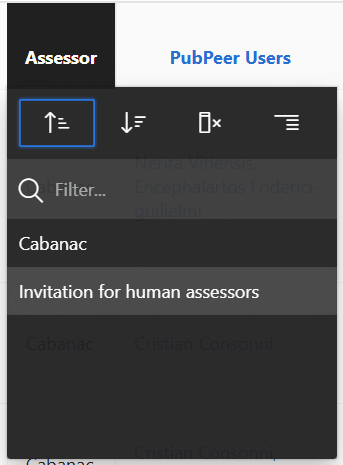
\includegraphics[width=0.3\linewidth]{img/getting_started/FilteringAssessors.png}

Existing PubPeer comments on articles are linked to in the `PubPeer Users' column. Existing PubPeer comments may be unrelated to the signature detected by the PPS (articles that contain problematic fingerprints likely feature other issues).

Just as you can filter for publishers or venues, you can show articles that still require manual assessment:

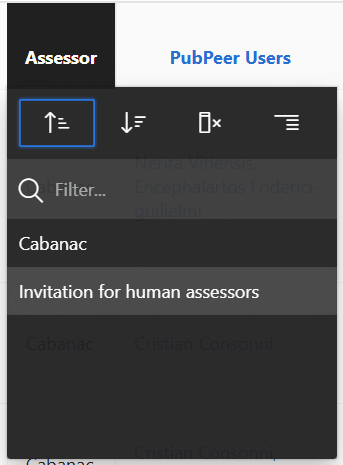
\includegraphics[width=0.3\linewidth]{img/getting_started/FilteringAssessors.png}

%Importantly, some of these may already have PubPeer comments as indicated in the rightmost column. Your job is to review the paper and post PubPeer comments if necessary, 

% Reese: is this how PPS works?
% after which a PPS administrator will double-check the comments and mark the paper as assessed.

To analyze an article flagged by the PPS and report problems with it:

\begin{enumerate}
    \setlength\itemsep{-0.5em}
    \item Click on the ``Tips'' cell for that article to open a popup that details the fingerprints the PPS found.
    \item Click on the ``Paper'' link in that popup to open the publisher's page for that article.
    \item Find the PPS-reported signatures within the article and examine their context. Keep an eye out for other issues that PPS might not be equipped to detect.
    \item Return to the PPS popup and click on the ``Copy comment to clipboard and open PubPeer'' button at the top.
    \item On PubPeer, click on the article's name to open its comment page and paste the copied template into the comment box.
    \item Take at least one screenshot of relevant section within the article and paste it in the comment to replace the placeholder text (you can paste images in the PubPeer text box and they will uploaded to PubPeer). Also consider copying the relevant section of the article and pasting it into the comment as a quotation (preceded by ``$>$'' in PubPeer's \href{https://pubpeer.com/static/markdown}{Markdown} language) with problematic sections bolded (two asterisks on either side in Markdown, e.g., **bold text**).
    \item Add anything else to the comment that adds useful information, such as other problems you've spotted within the quoted sections.
    \item Preview before submitted to ensure that the comment is formatted correctly, then post!
\end{enumerate}

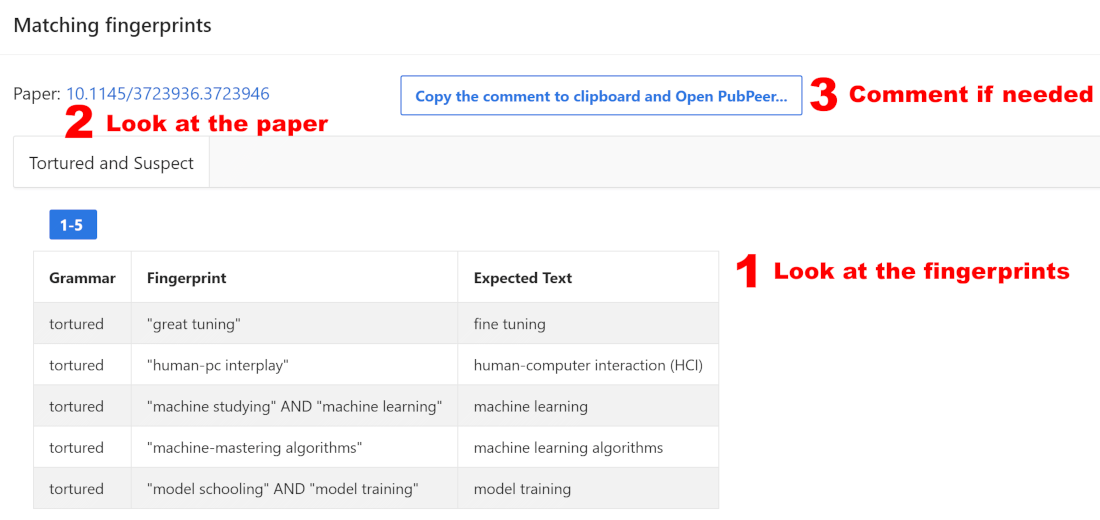
\includegraphics[width=\linewidth]{img/getting_started/process_reduced.png}

PPS admins continuously assess new PubPeer comments to add new fingerprints to the PPS and evaluate existing fingerprints. Further information on the PPS can be found on its \href{https://www.irit.fr/~Guillaume.Cabanac/problematic-paper-screener/faq}{FAQ page}. This page features examples on how to navigate on the PPS and the names of some prolific PubPeer commentators to get ideas on how to comment.

\subsection*{Begin with what you know}

Although anyone can perform PPPR with the right domain knowledge (which COSIG aims to distribute) the best-prepared are working scientists reviewing papers in their career discipline. If you are a working scientist, consider starting by reviewing articles in your field, especially if you have already noticed issues. Some prolific PPPR practioners, often called ``sleuths'', began after noticing that their own work was \href{https://osf.io/ntcb4}{plagiarized}. Others began after noticing that an article they read as part of a ``journal club'' in their laboratory contained \href{https://osf.io/547re}{duplicated images}.

Consider limiting your PPPR activity to just one or two issues when you first start (such as one of the fingerprints collected by the PPS), acquiring an eye for other issues along the way.

Finding one problematic article tends to lead to finding other, related problematic articles. Once you've reviewed one article, consider looking at other articles in the same publication venue or by the same authors.

\subsection*{Learn from others}

It is always worthwhile to read \href{https://pubpeer.com/recent/}{recent} and \href{https://pubpeer.com/}{moderator-selected} PubPeer comments to learn how others are using the site. PubPeer comments can also provide leads on particular topics and publication venues that are worth further examination.

If you identify an unfamiliar issue in an article, consider searching PubPeer to see if anyone else has identified a similar issue elsewhere--this may give you an idea for how to frame the problem in your comment.

\subsection*{Additional resources}

\begin{itemize}
    \setlength\itemsep{-0.5em}
    \item \href{https://osf.io/sghaq}{COSIG: PubPeer commenting best practices}
    \item \href{https://doi.org/10.5281/zenodo.14871842}{\textit{An Introduction to Forensic Metascience}}
\end{itemize}

\end{document}